\documentclass[11pt,preprint, authoryear]{elsarticle}

\usepackage{lmodern}
%%%% My spacing
\usepackage{setspace}
\setstretch{1.2}
\DeclareMathSizes{12}{14}{10}{10}

% Wrap around which gives all figures included the [H] command, or places it "here". This can be tedious to code in Rmarkdown.
\usepackage{float}
\let\origfigure\figure
\let\endorigfigure\endfigure
\renewenvironment{figure}[1][2] {
    \expandafter\origfigure\expandafter[H]
} {
    \endorigfigure
}

\let\origtable\table
\let\endorigtable\endtable
\renewenvironment{table}[1][2] {
    \expandafter\origtable\expandafter[H]
} {
    \endorigtable
}


\usepackage{ifxetex,ifluatex}
\usepackage{fixltx2e} % provides \textsubscript
\ifnum 0\ifxetex 1\fi\ifluatex 1\fi=0 % if pdftex
  \usepackage[T1]{fontenc}
  \usepackage[utf8]{inputenc}
\else % if luatex or xelatex
  \ifxetex
    \usepackage{mathspec}
    \usepackage{xltxtra,xunicode}
  \else
    \usepackage{fontspec}
  \fi
  \defaultfontfeatures{Mapping=tex-text,Scale=MatchLowercase}
  \newcommand{\euro}{€}
\fi

\usepackage{amssymb, amsmath, amsthm, amsfonts}

\def\bibsection{\section*{References}} %%% Make "References" appear before bibliography


\usepackage[round]{natbib}

\usepackage{longtable}
\usepackage[margin=2.3cm,bottom=2cm,top=2.5cm, includefoot]{geometry}
\usepackage{fancyhdr}
\usepackage[bottom, hang, flushmargin]{footmisc}
\usepackage{graphicx}
\numberwithin{equation}{section}
\numberwithin{figure}{section}
\numberwithin{table}{section}
\setlength{\parindent}{0cm}
\setlength{\parskip}{1.3ex plus 0.5ex minus 0.3ex}
\usepackage{textcomp}
\renewcommand{\headrulewidth}{0.2pt}
\renewcommand{\footrulewidth}{0.3pt}

\usepackage{array}
\newcolumntype{x}[1]{>{\centering\arraybackslash\hspace{0pt}}p{#1}}

%%%%  Remove the "preprint submitted to" part. Don't worry about this either, it just looks better without it:
\makeatletter
\def\ps@pprintTitle{%
  \let\@oddhead\@empty
  \let\@evenhead\@empty
  \let\@oddfoot\@empty
  \let\@evenfoot\@oddfoot
}
\makeatother

 \def\tightlist{} % This allows for subbullets!

\usepackage{hyperref}
\hypersetup{breaklinks=true,
            bookmarks=true,
            colorlinks=true,
            citecolor=blue,
            urlcolor=blue,
            linkcolor=blue,
            pdfborder={0 0 0}}


% The following packages allow huxtable to work:
\usepackage{siunitx}
\usepackage{multirow}
\usepackage{hhline}
\usepackage{calc}
\usepackage{tabularx}
\usepackage{booktabs}
\usepackage{caption}


\newenvironment{columns}[1][]{}{}

\newenvironment{column}[1]{\begin{minipage}{#1}\ignorespaces}{%
\end{minipage}
\ifhmode\unskip\fi
\aftergroup\useignorespacesandallpars}

\def\useignorespacesandallpars#1\ignorespaces\fi{%
#1\fi\ignorespacesandallpars}

\makeatletter
\def\ignorespacesandallpars{%
  \@ifnextchar\par
    {\expandafter\ignorespacesandallpars\@gobble}%
    {}%
}
\makeatother

\newenvironment{CSLReferences}[2]{%
}

\urlstyle{same}  % don't use monospace font for urls
\setlength{\parindent}{0pt}
\setlength{\parskip}{6pt plus 2pt minus 1pt}
\setlength{\emergencystretch}{3em}  % prevent overfull lines
\setcounter{secnumdepth}{5}

%%% Use protect on footnotes to avoid problems with footnotes in titles
\let\rmarkdownfootnote\footnote%
\def\footnote{\protect\rmarkdownfootnote}
\IfFileExists{upquote.sty}{\usepackage{upquote}}{}

%%% Include extra packages specified by user

%%% Hard setting column skips for reports - this ensures greater consistency and control over the length settings in the document.
%% page layout
%% paragraphs
\setlength{\baselineskip}{12pt plus 0pt minus 0pt}
\setlength{\parskip}{12pt plus 0pt minus 0pt}
\setlength{\parindent}{0pt plus 0pt minus 0pt}
%% floats
\setlength{\floatsep}{12pt plus 0 pt minus 0pt}
\setlength{\textfloatsep}{20pt plus 0pt minus 0pt}
\setlength{\intextsep}{14pt plus 0pt minus 0pt}
\setlength{\dbltextfloatsep}{20pt plus 0pt minus 0pt}
\setlength{\dblfloatsep}{14pt plus 0pt minus 0pt}
%% maths
\setlength{\abovedisplayskip}{12pt plus 0pt minus 0pt}
\setlength{\belowdisplayskip}{12pt plus 0pt minus 0pt}
%% lists
\setlength{\topsep}{10pt plus 0pt minus 0pt}
\setlength{\partopsep}{3pt plus 0pt minus 0pt}
\setlength{\itemsep}{5pt plus 0pt minus 0pt}
\setlength{\labelsep}{8mm plus 0mm minus 0mm}
\setlength{\parsep}{\the\parskip}
\setlength{\listparindent}{\the\parindent}
%% verbatim
\setlength{\fboxsep}{5pt plus 0pt minus 0pt}



\begin{document}



\begin{frontmatter}  %

\title{Movies}

% Set to FALSE if wanting to remove title (for submission)




\author[Add1]{Gabriella Neilon}
\ead{22581340@sun.ac.za}





\address[Add1]{Stellenbosch University}

\cortext[cor]{Corresponding author: Gabriella Neilon}

\begin{abstract}
\small{
Abstract to be written here. This will look at Movies.
}
\end{abstract}

\vspace{1cm}


\begin{keyword}
\footnotesize{
Multivariate GARCH \sep Kalman Filter \sep Copula \\
\vspace{0.3cm}
}
\footnotesize{
\textit{JEL classification} L250 \sep L100
}
\end{keyword}



\vspace{0.5cm}

\end{frontmatter}

\setcounter{footnote}{0}



%________________________
% Header and Footers
%%%%%%%%%%%%%%%%%%%%%%%%%%%%%%%%%
\pagestyle{fancy}
\chead{}
\rhead{}
\lfoot{}
\rfoot{\footnotesize Page \thepage}
\lhead{}
%\rfoot{\footnotesize Page \thepage } % "e.g. Page 2"
\cfoot{}

%\setlength\headheight{30pt}
%%%%%%%%%%%%%%%%%%%%%%%%%%%%%%%%%
%________________________

\headsep 35pt % So that header does not go over title




\hypertarget{introduction}{%
\section{\texorpdfstring{Introduction
\label{Introduction}}{Introduction }}\label{introduction}}

References are to be made as follows: Fama \& French
(\protect\hyperlink{ref-fama1997}{1997: 33}) and Grinold \& Kahn
(\protect\hyperlink{ref-grinold2000}{2000}) Such authors could also be
referenced in brackets (\protect\hyperlink{ref-grinold2000}{Grinold \&
Kahn, 2000}) and together Grinold \& Kahn
(\protect\hyperlink{ref-grinold2000}{2000}). Source the reference code
from scholar.google.com by clicking on ``cite'\,' below article name.
Then select BibTeX at the bottom of the Cite window, and proceed to copy
and paste this code into your ref.bib file, located in the directory's
Tex folder. Open this file in Rstudio for ease of management, else open
it in your preferred Tex environment. Add and manage your article
details here for simplicity - once saved, it will self-adjust in your
paper.

\begin{quote}
I suggest renaming the top line after @article, as done in the template
ref.bib file, to something more intuitive for you to remember. Do not
change the rest of the code. Also, be mindful of the fact that bib
references from google scholar may at times be incorrect. Reference
Latex forums for correct bibtex notation.
\end{quote}

To reference a section, you have to set a label using
``\textbackslash label'\,' in R, and then reference it in-text as
e.g.~referencing a later section, Section \ref{Meth}.

Writing in Rmarkdown is surprizingly easy - see
\href{https://www.rstudio.com/wp-content/uploads/2015/03/rmarkdown-reference.pdf}{this
website} cheatsheet for a summary on writing Rmd writing tips.

\hypertarget{data}{%
\section*{Data}\label{data}}
\addcontentsline{toc}{section}{Data}

Notice how I used the curly brackets and dash to remove the numbering of
the data section.

Discussion of data should be thorough with a table of statistics and
ideally a figure.

In your tempalte folder, you will find a Data and a Code folder. In
order to keep your data files neat, store all of them in your Data
folder. Also, I strongly suggest keeping this Rmd file for writing and
executing commands, not writing out long pieces of data-wrangling. In
the example below, I simply create a ggplot template for scatter plot
consistency. I suggest keeping all your data in a data folder.

To make your graphs look extra nice in latex world, you could use Tikz
device. Replace dev - `png' with `tikz' in the chunk below. Notice this
makes the build time longer and produces extra tex files - so if you are
comfortable with this, set your device to Tikz and try it out:

To reference the plot above, add a ``\textbackslash label'\,' after the
caption in the chunk heading, as done above. Then reference the plot as
such: As can be seen, Figures \ref{Figure1} and \ref{Figure2} are
excellent, with Figure \ref{Figure2} being particularly aesthetically
pleasing due to its device setting of Tikz. The nice thing now is that
it correctly numbers all your figures (and sections or tables) and will
update if it moves. The links are also dynamic.

I very strongly suggest using ggplot2 (ideally in combination with
dplyr) using the ggtheme package to change the themes of your figures.

Also note the information that I have placed above the chunks in the
code chunks for the figures. You can edit any of these easily - visit
the Rmarkdown webpage for more information.

\hypertarget{splitting-a-page}{%
\section{Splitting a page}\label{splitting-a-page}}

You can also very easily split a page using built-in Pandoc formatting.
I comment this out in the code (as this has caused issues building the
pdf for some users - which I presume to be a Pandoc issue), but you are
welcome to try it out yourself by commenting out the following section
in your Rmd file.

\hypertarget{results}{%
\section{Results}\label{results}}

\#First statement ``I firmly remember that Rotten Tomatoes was always a
great review platform - and if a movie had a rating of more than 80\% on
Rotten Tomatoes, audiences would rate it above 85\% every time.''

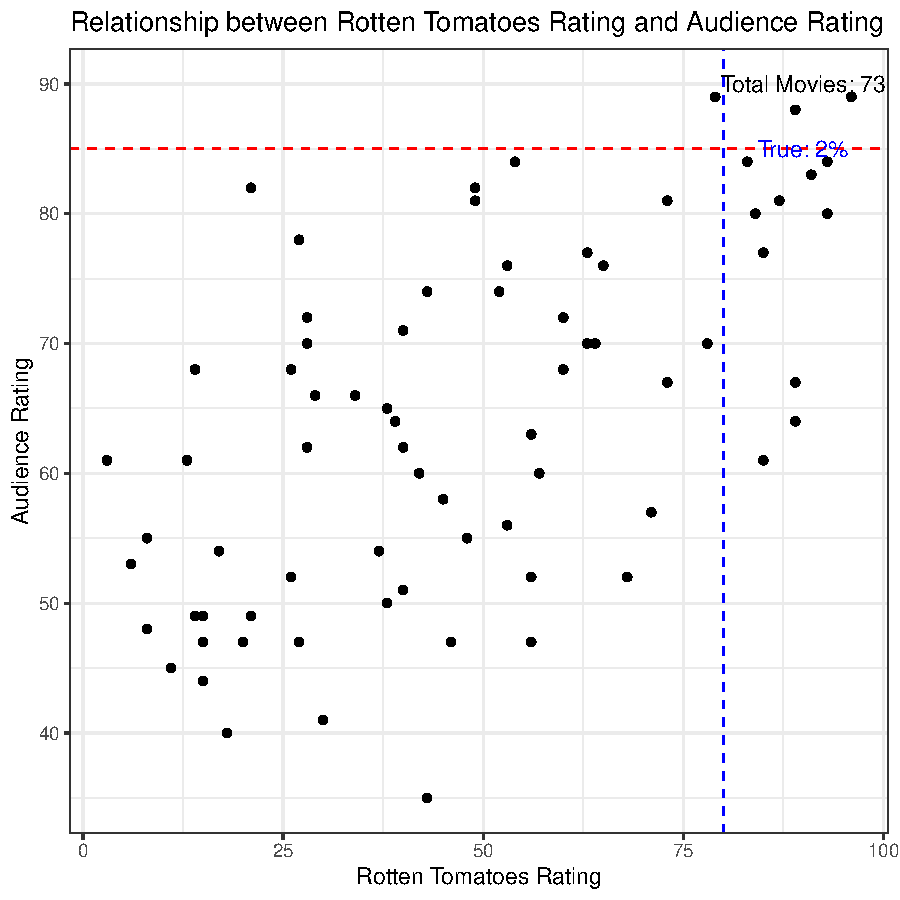
\includegraphics{Project_Question3_files/figure-latex/unnamed-chunk-1-1.pdf}

\#Statment 2 ``Disney films may not have the highest grossing numbers,
but they've always been the most profitable of all the leading studios''

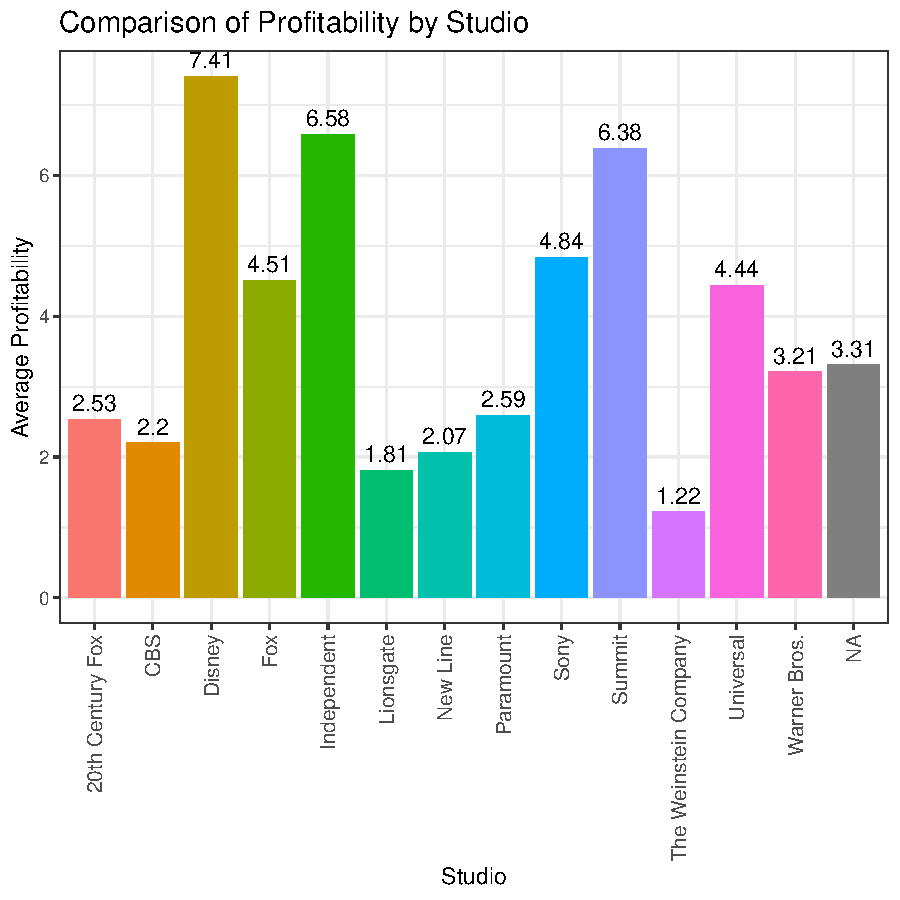
\includegraphics{Project_Question3_files/figure-latex/unnamed-chunk-2-1.pdf}

\#Statement 3: ``Audiences are always drawn to the highest grossing
films. In fact, I bet the correlation between the world wide grossing
numbers and audience scores would be near 80\%.''

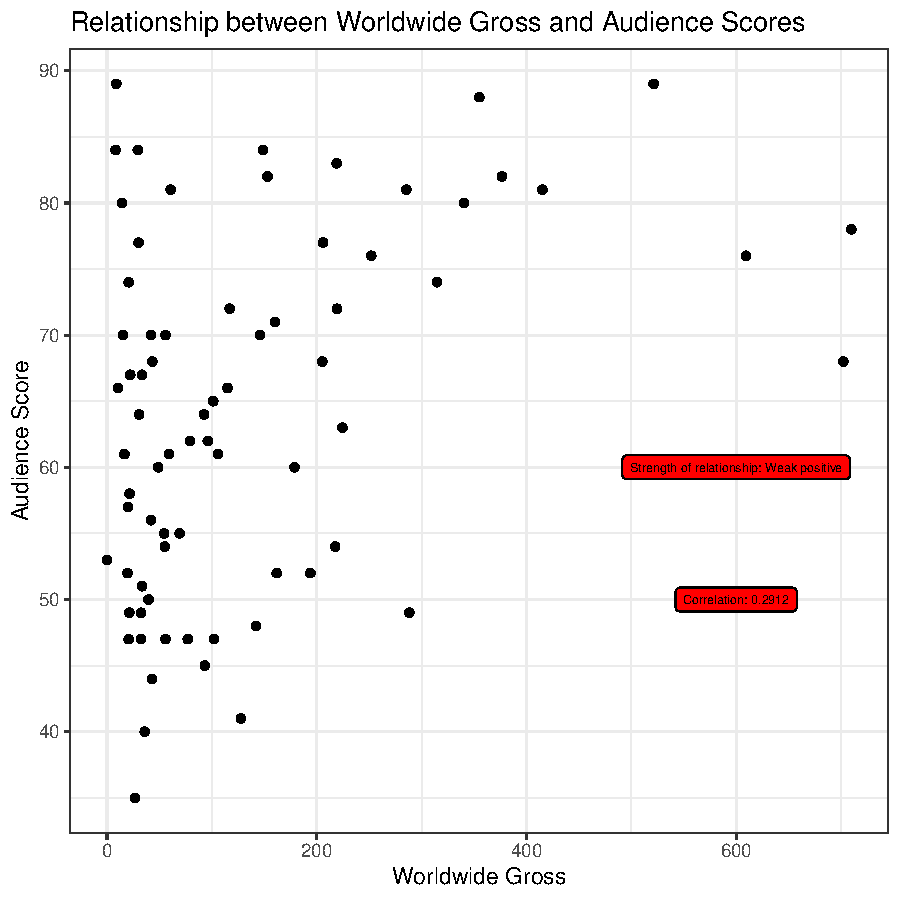
\includegraphics{Project_Question3_files/figure-latex/unnamed-chunk-3-1.pdf}

\hfill

\hypertarget{conclusion}{%
\section{Conclusion}\label{conclusion}}

I hope you find this template useful. Remember, stackoverflow is your
friend - use it to find answers to questions. Feel free to write me a
mail if you have any questions regarding the use of this package. To
cite this package, simply type citation(``Texevier'') in Rstudio to get
the citation for Katzke (\protect\hyperlink{ref-Texevier}{2017}) (Note
that uncited references in your bibtex file will not be included in
References).

\newpage

\hypertarget{references}{%
\section*{References}\label{references}}
\addcontentsline{toc}{section}{References}

\hypertarget{refs}{}
\begin{CSLReferences}{1}{0}
\leavevmode\vadjust pre{\hypertarget{ref-fama1997}{}}%
Fama, E.F. \& French, K.R. 1997. Industry costs of equity. \emph{Journal
of financial economics}. 43(2):153--193.

\leavevmode\vadjust pre{\hypertarget{ref-grinold2000}{}}%
Grinold, R.C. \& Kahn, R.N. 2000. Active portfolio management.

\leavevmode\vadjust pre{\hypertarget{ref-Texevier}{}}%
Katzke, N.F. 2017. \emph{{Texevier}: {P}ackage to create elsevier
templates for rmarkdown}. Stellenbosch, South Africa: Bureau for
Economic Research.

\end{CSLReferences}

\bibliography{Tex/ref}





\end{document}
